\chapter[Some Recollection]{Some Recollections\footnote[*]{Address by Prof.\ G Ramachandran on the occasion of Golden Jubilee of The Institute of Mathematical Sciences, 3 January 2012.}}\label{chap2}

\Authorline{G Ramachandran}
\addtocontents{toc}{\protect\contentsline{section}{{\sl G Ramachandran}\smallskip}{}}
\medskip

Let me thank Professor Ghanashyam Date for inviting me and Professor M V N Murthy
for agreeing to present some of my recollections on my behalf.

I was at the Institute of Mathematical Sciences in the first three years of the
Institute [after its inauguration], during which I was given an opportunity to give
a Course of Lectures on the Quantum Theory of Angular Momentum and to assist
in guiding Dr.\ K Ananthanarayanan and Late Dr.\ R K Umerjee. The work with Dr.\ 
Ananthanarayanan was appreciated by Late Professor L I Schiff, while the work with
Dr.\ Umerjee led me much later to the realization of what Professor Murthy and I
referred to as Non-Oriented Spin Systems and to the beautiful SU(n) representation
[of the density matrix of arbitrary spin systems] proposed by us. The early work
carried out by Professor V Devanathan and myself here [in Madras] on photo-pion
production motivated me to formulate a new method, during the first decade of
this century, to derive the multipole expansions for photo-production and electro-
production of mesons with arbitrary spin-parities at higher energies in collaboration
with Dr.\ M S Vidya and Professor J Balasubramanyam. These new results specialize
exactly to the corresponding CGLN [Chew, Goldberger, Low and Nambu] expansions
in the particularly simple case of pseudo-scalar mesons

The exhortation that research is best done when it is part of a way of life, by
my teacher Late Professor Alladi Ramakrishnan, has all along influenced me. The
frequent meetings with eminent scientists, which were highly inspiring, right from
the time I joined as a student was given an identity when he created the Theoretical
Physics Seminar on Sri Rama Navami in 1959. I was a Member from its inception.
Apart from the tireless work and the emotional attachment to the cause of\break 
Theoretical physics, we contributed money too, in the form of the Membership fee paid every
month and additional payments for all the dinners and buffet parties without exception. 
The List of Members is attached. I also had the privilege of giving a Course
of Lectures on Nuclear Physics to the first batch of M Sc Nuclear Physics students
comprising Professor A P Balachandran, Professor G Bhamathi, Dr.\ T K Radha and
Dr.\ R Thunga.

Finally I wish to record the advice, ``You have taken a step forward; don’t take it
back", given early at a very difficult time by my father Late Sri Gowravaram Venkata
Krishnaiah (G V K) garu.

It was crucial for my continuation in research, which was given a new life by the
great scientist Dr.\ C R Rao F R S and my dear friend Dr.\ B Ramachandran F N A at
the end of my tenure at MATSCIENCE (I M Sc).

\hfill
Thank you.

\begin{figure}[H]
\centering
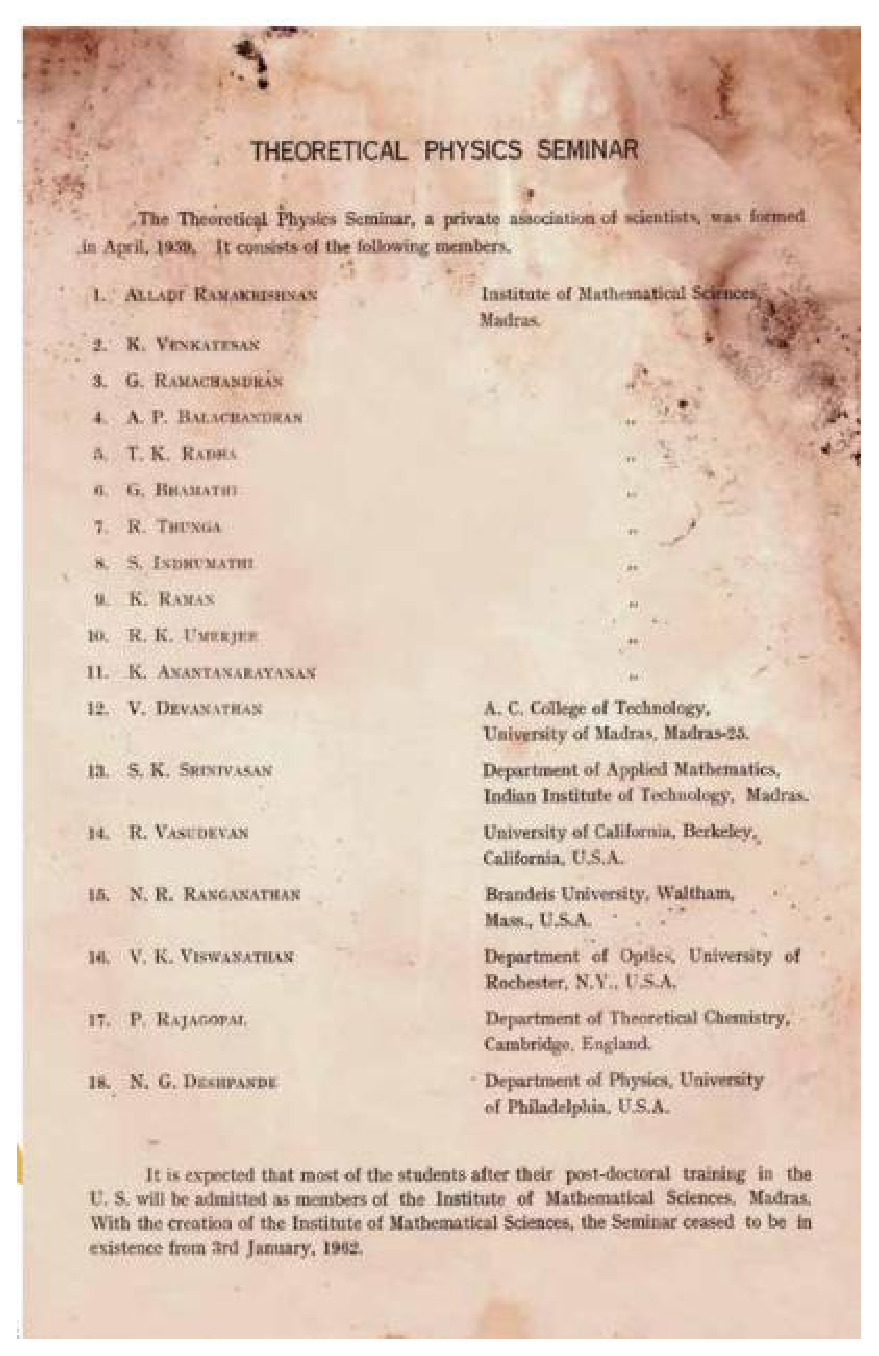
\includegraphics[scale=0.65]{src/images/chap25/1.eps}
\caption{List of members of Theoretical Physics Seminar started in April 1959. Matscience grew out of
this Association on January 3, 1962.}
\end{figure}

\eject

\begin{center}
{\bf \Large Memories of GR at IMSc}
\end{center}

\begin{figure}[H]
\centering
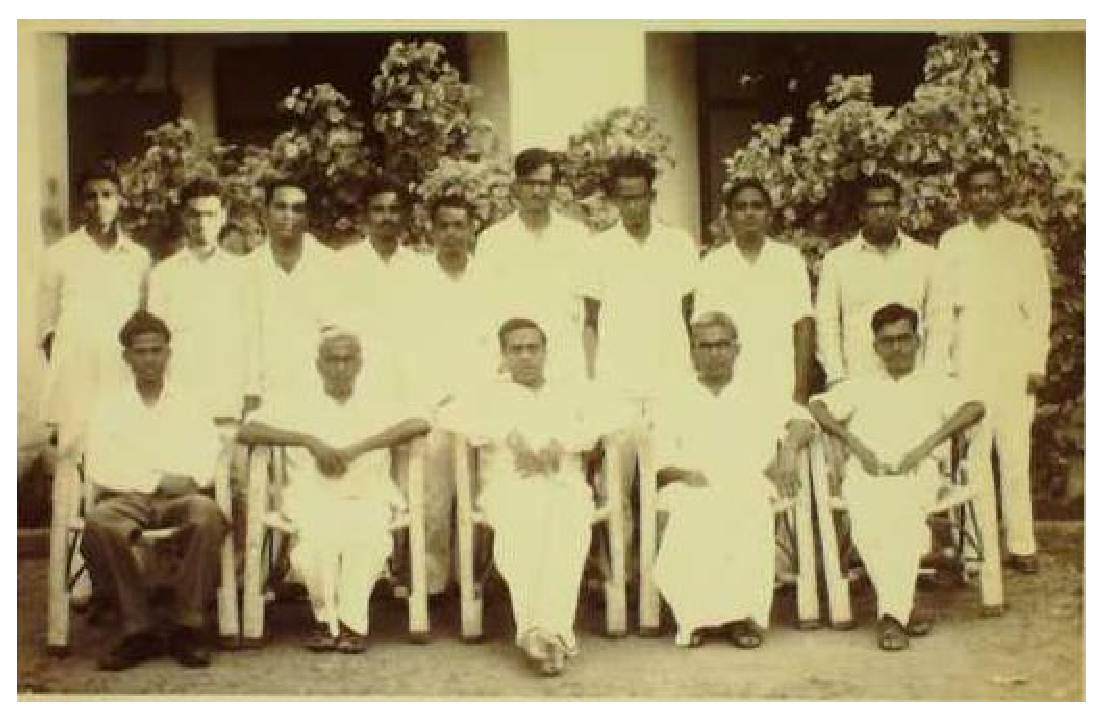
\includegraphics[scale=0.33]{src/images/chap25/2.eps}
\caption{Members of Theoretical Physics Seminar. Alladi\break Ramakrishnan is seated
in the middle, GR is standing fourth from left.}
\end{figure}
\medskip

\begin{figure}[H]
\centering
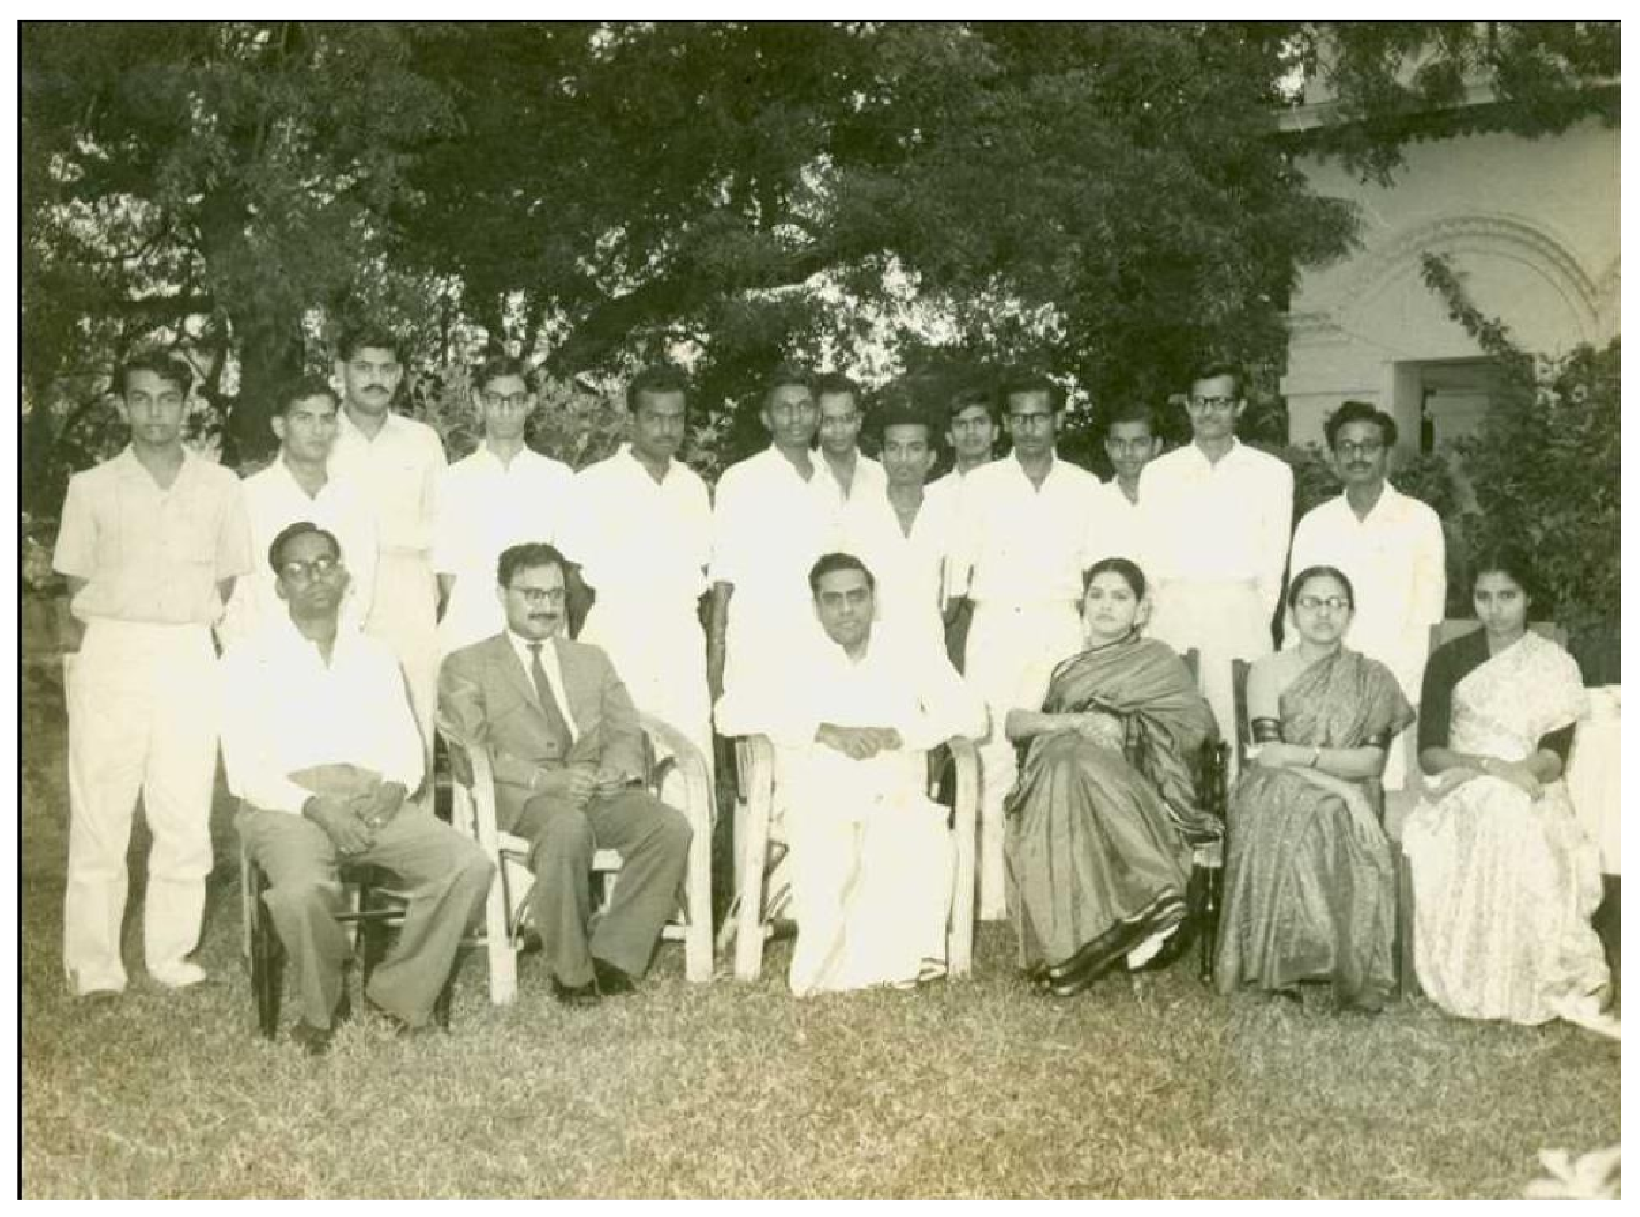
\includegraphics[scale=0.33]{src/images/chap25/3.eps}
\caption{During a visit by Prof.\ Abdus Salam. Sitting: Dr.\ S K\break Srinivasan, Dr.\ Abdus Salam, 
Dr.\ Alladi Ramakrishnan, Mrs.\break Ramakrishnan, R Thunga, T K Radha. 
V Devanathan and G\break Ramachandran are standing to the right extreme.}
\end{figure}

\begin{figure}[H]
\centering
\includegraphics[scale=0.34]{src/images/chap25/4.eps}
\caption{During a visit by Donald Glaser. First row: R Thunga,
T K Radha, Donald Glaser, Alladi Ramakrishnan, S Indumathi, 
G Bhamathi. Back row: A P Balachandran (first person), the last two persons are V Devanathan and G Ramachandran.}
\end{figure}
\medskip

\begin{figure}[H]
\centering
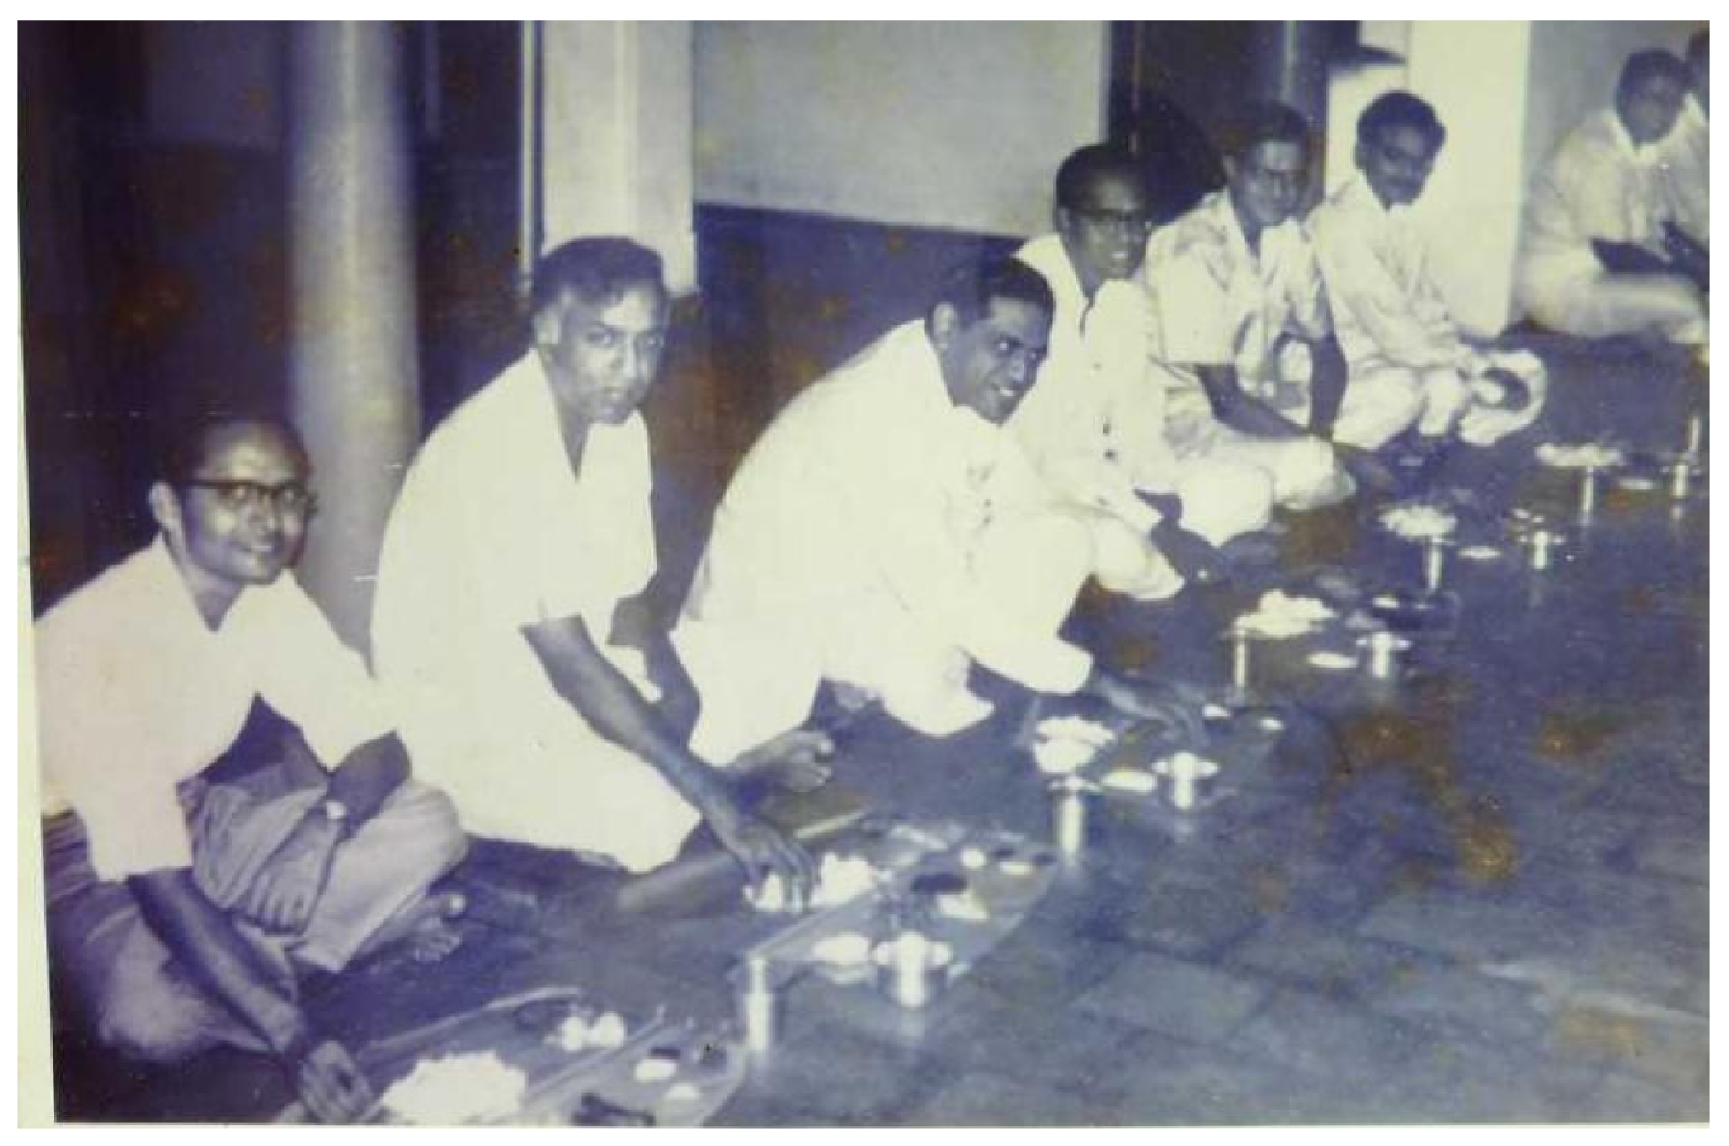
\includegraphics[scale=0.34]{src/images/chap25/5.eps}
\caption{Having a South Indian lunch with S Chandrasekhar. From left, A P
Balachandran, S Chandrasekhar, Alladi Ramakrishnan,\break unknown, V Devanathan, G
Ramachandran.}
\end{figure}

\begin{figure}[H]
\centering
\includegraphics[scale=0.35]{src/images/chap25/6.eps}
\caption{TIFR Bangalore summer school in 1961, where Gellmann lectured on the
quark model for the first time. GR is standing in the second row, second from left
next to A P Balachandran. Indumathi and Radha are standing in front of them where
as Thunga and Bhamathi are seen standing at right. Homi Bhabha is standing in
the middle flanked by M G K Menon and Gellmann to his right, Dalitz and Alladi\break
Ramakrishnan to his left.}
\end{figure}


